\documentclass[utf8,xcolor=table]{beamer}

\usepackage[T2A]{fontenc}
\usepackage[utf8]{inputenc}
\usepackage[english,russian]{babel}
%\usepackage{tikz-uml}
%\usepackage{minted}

\mode<presentation>{
	\usetheme{CambridgeUS}
}

\renewcommand{\t}[1]{\ifmmode{\mathtt{#1}}\else{\texttt{#1}}\fi}

\title{Оффлайн-просмотр ленты ВК}
\author{Егор Суворов}
\institute[СПб АУ]{Практика, осень 2015\\Какой такой куратор?}
\date[18.12.2015]{Пятница, 18 декабря 2015 года}

\setlength{\arrayrulewidth}{1pt}

\begin{document}

\begin{frame}
\titlepage
\end{frame}

\begin{frame}[t]{Мотивация}
	\begin{itemize}
		\item В мире много мест с плохой связью, где приходится чем-то занимать время
		\item Лента ВК занимает всё доступное время, но без интернета её не полистать
		\item Официальные клиенты не умеют активно всё кэшировать и при обрыве связи могут выкинуть половину загруженного непосильным трудом
		\item Кажется, что никто не умеет скачивать веб-страницы, приложенные к записям в ленте
	\end{itemize}
\end{frame}

\begin{frame}[t]{Задачи}
	\begin{itemize}
		\item Агрессивное кэширование, даже если какие-то фрагменты ленты остаются неподгруженными
		\item Подгрузка ленты с любого места по запросу
		\item Автоматическое скачивание веб-страниц, на которые ссылаются записи (с зависимостями)
		\item Можно отключить интернет, закрыть приложение, зайти обратно и ничего не потерять
	\end{itemize}
\end{frame}

\begin{frame}[t]{Пример разрыва ленты}
	\begin{center}
		\begin{tabular}{ccc}
			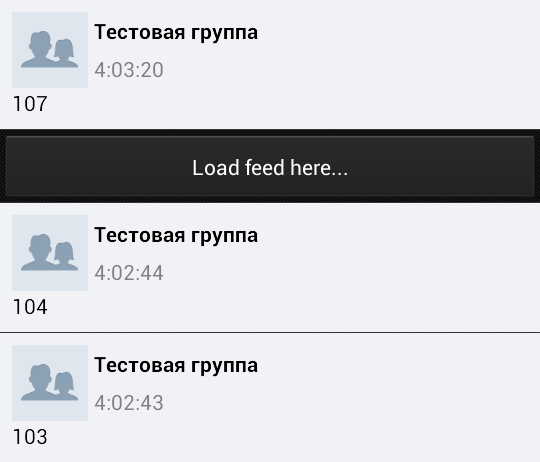
\includegraphics[scale=0.18]{a.png}
			&
			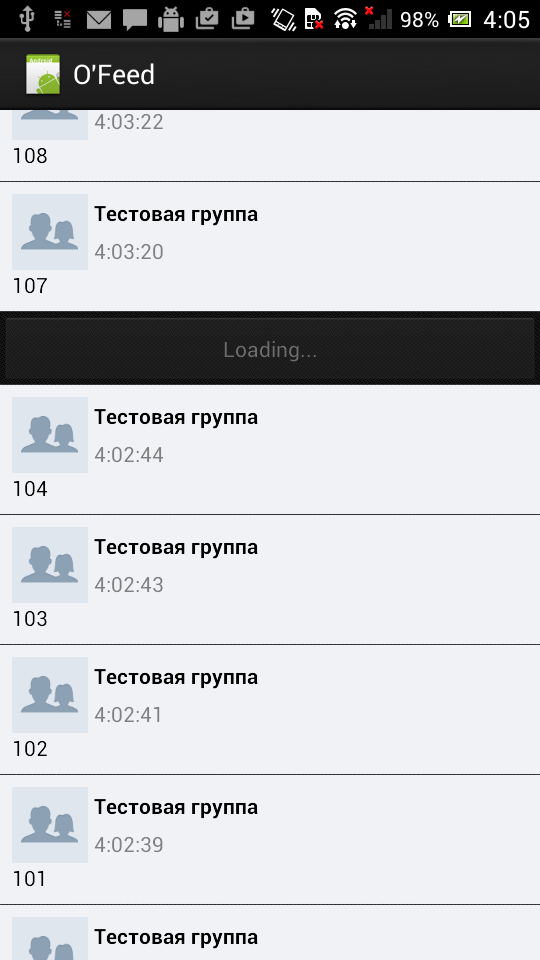
\includegraphics[scale=0.18]{b.png}
			&
			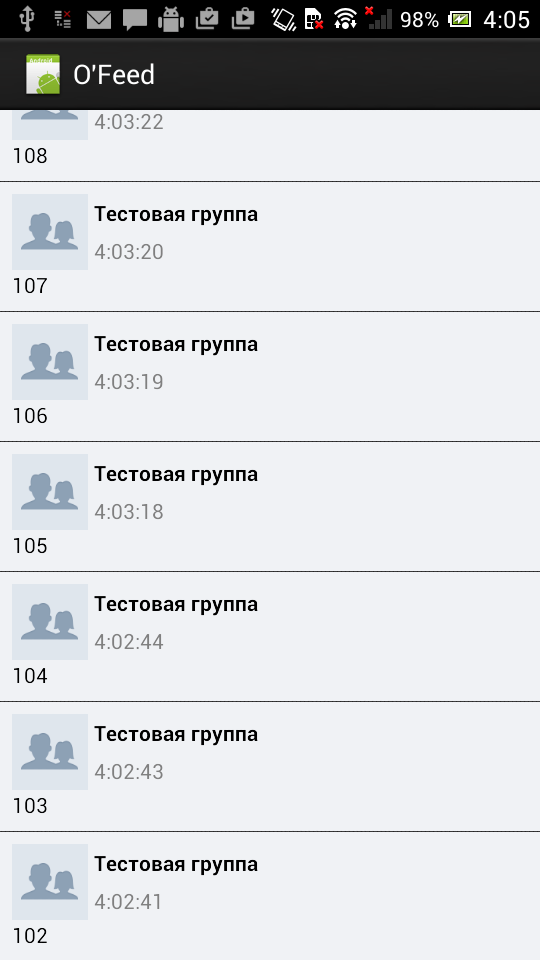
\includegraphics[scale=0.18]{c.png}
		\end{tabular}
	\end{center}
\end{frame}

\begin{frame}[t]{Используемые библиотеки}
	\begin{itemize}
		\item ORMLite "--- общение с базой данных (SQLite), где хранятся все данные и информация про кэшированные файлы
		\item JSoup "--- парсинг и изменение HTML
		\item VK Android Library "--- взаимодействие с VK API (местами дописана самостоятельно)
	\end{itemize}
\end{frame}

\begin{frame}[t]{Схема загрузки веб-страниц}
	\begin{enumerate}
		\item Страница загружается в общедоступное место на карте памяти
		\item Ищутся ресурсы: CSS-файлы и картинки
		\item Исходная страница перезаписывается так, чтобы все ссылки указывали на локальную файловую систему
		\item Начинается параллельная загрузка ресурсов
		\item После окончания всех загрузок страница помечается, как закэшированная
	\end{enumerate}
\end{frame}

\begin{frame}[t]{Схема хранения фрагментов ленты}
	У каждого элемента ленты есть два состояния:
	\begin{enumerate}
		\item С этим элементом был загружен некоторый следующий элемент
		\item Этот элемент был последним в своём запросе и ВК вернул указатель на следующую <<страницу>>
	\end{enumerate}
	Также в БД для упрощения взаимодействия с адаптерами хранятся заглушки, указывающие на конец
	загруженной <<страницы>> новостей.

	При загрузке очередного фрагмента надо:
	\begin{itemize}
		\item У некоторых элементов поставить флаг <<есть следующий>>
		\item Убрать заглушки, стоящие после таких элементов
		\item Возможно, добавить одну новую заглушку
	\end{itemize}
\end{frame}

\begin{frame}[t]{Сложные места}
	\begin{enumerate}
		\item Отсутствие в VK Android Library классов для работы с лентой новостей
		\item Открытие HTML-файла с локального диска в браузере
		\item Адаптер для ListView для прокрутки длинных списков с возможностью догрузки в процессе
		\item Сериализация объектов VK Android Library в SQLite (увы, Parcelable)
		\item Собственные View для отображения постов и вложений
	\end{enumerate}
\end{frame}

\begin{frame}[t]{Ссылки}
  \begin{itemize}
  \item \href{mailto:egor_suvorov@mail.ru}{\t{egor\_suvorov@mail.ru}}
  \item \href{http://github.com/yeputons/ofeed/}{\t{github.com/yeputons/ofeed}}
  \item \href{http://yeputons.net/pub/ofeed.apk}{\t{yeputons.net/pub/ofeed.apk}}
  \end{itemize}
\end{frame}

\end{document}
